\documentclass[12pt]{article}
\setlength{\headheight}{14.5pt}
\addtolength{\topmargin}{-2.5pt}

\usepackage{pgfplots} % Add this line to include the pgfplots package
\usepackage{amsmath}
\usepackage{geometry}
\usepackage{setspace}
\usepackage{graphicx}
\usepackage{fancyhdr}
\usepackage{xcolor}
\usepackage{titlesec}
\usepackage{booktabs}
\usepackage{hyperref}
\usepackage{soul}
\usepackage{wrapfig}
\usepackage{placeins}
\usepackage{float}
 


\hypersetup{
    colorlinks=true,       % Enable colored links
    linkcolor=blue,        % Color of internal links
    filecolor=magenta,     % Color of file links
    urlcolor=cyan          % Color of external links
}



\renewcommand{\headrulewidth}{0pt} % Remove header rule
\renewcommand{\footrulewidth}{0pt} % Remove footer rule




\usepackage{url}
\geometry{a4paper, margin=0.7in }
\setlength{\parindent}{0pt}
\setstretch{1.5}
\usepackage{setspace}
% Header and Footer
\usepackage{fancyhdr}
\pagestyle{fancy}
\fancyhf{} % Clear all header and footer fields
\fancyhead[L]{\textbf{19-AIBM4}} % Top-left text
\fancyhead[C]{\rule{\textwidth}{0.5pt}} % Top horizontal line

% Combine the page numbering and horizontal rule into one footer definition
\fancyfoot[C]{\rule{\textwidth}{0.5pt}\\ Page \thepage\ of 15} % Bottom horizontal line with page number


% Title formatting
\titleformat{\section}[block]
  {\large\bfseries\sffamily\color{red}}
  {\thesection.}{1em}{}

\titleformat{\subsection}[block]
  {\normalsize\bfseries\sffamily\color{red}}
  {\thesubsection}{1em}{}
 \pgfplotsset{compat=1.18} 
\begin{document}


\pagenumbering{arabic} % Ensure Arabic numbering starts from the first page



 
% -------------------------------------------------------------
% COVER PAGE
% -------------------------------------------------------------
\begin{titlepage}
\centering
% University logo or other image

\includegraphics[width=0.4\textwidth]{UoD_Engineering.jpg} \\
\vspace{10mm}

% Title and subtitle
{\LARGE \textbf{Feasibility Report for Group 19-AIBM4 Autonomous Material Mover}} \\[10pt]

\vspace{5mm}\hrule\vspace{0mm}

% Insert image with caption for the material mover
\begin{figure}[h!]
    \centering
     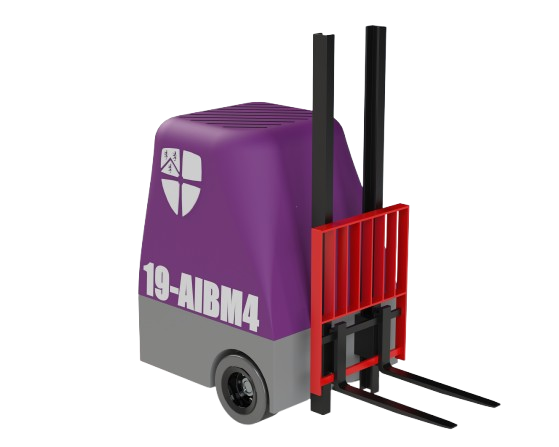
\includegraphics[width=1\textwidth]{Pooled_Design_V2__6_-removebg-preview.png}
\end{figure}  
\vspace{0mm}
\vspace{10mm}

% Title and author block
{\large \textbf{Co-Authors: }\textit{A Wright, A Wigmore, H Billing, J Wang, L Nangle, W Woodward}} \\ \vspace{1mm}
{Supervisors:\textit{ Dr Aissa Ikhlef, Bill Maxwell}} \\[10pt]
{\small The University of Durham \\ \today}
\end{titlepage}

% -------------------------------------------------------------
% FRONTMATTER
% -------------------------------------------------------------
\tableofcontents
%\begin{figure}[h!]
 %   \centering
 %    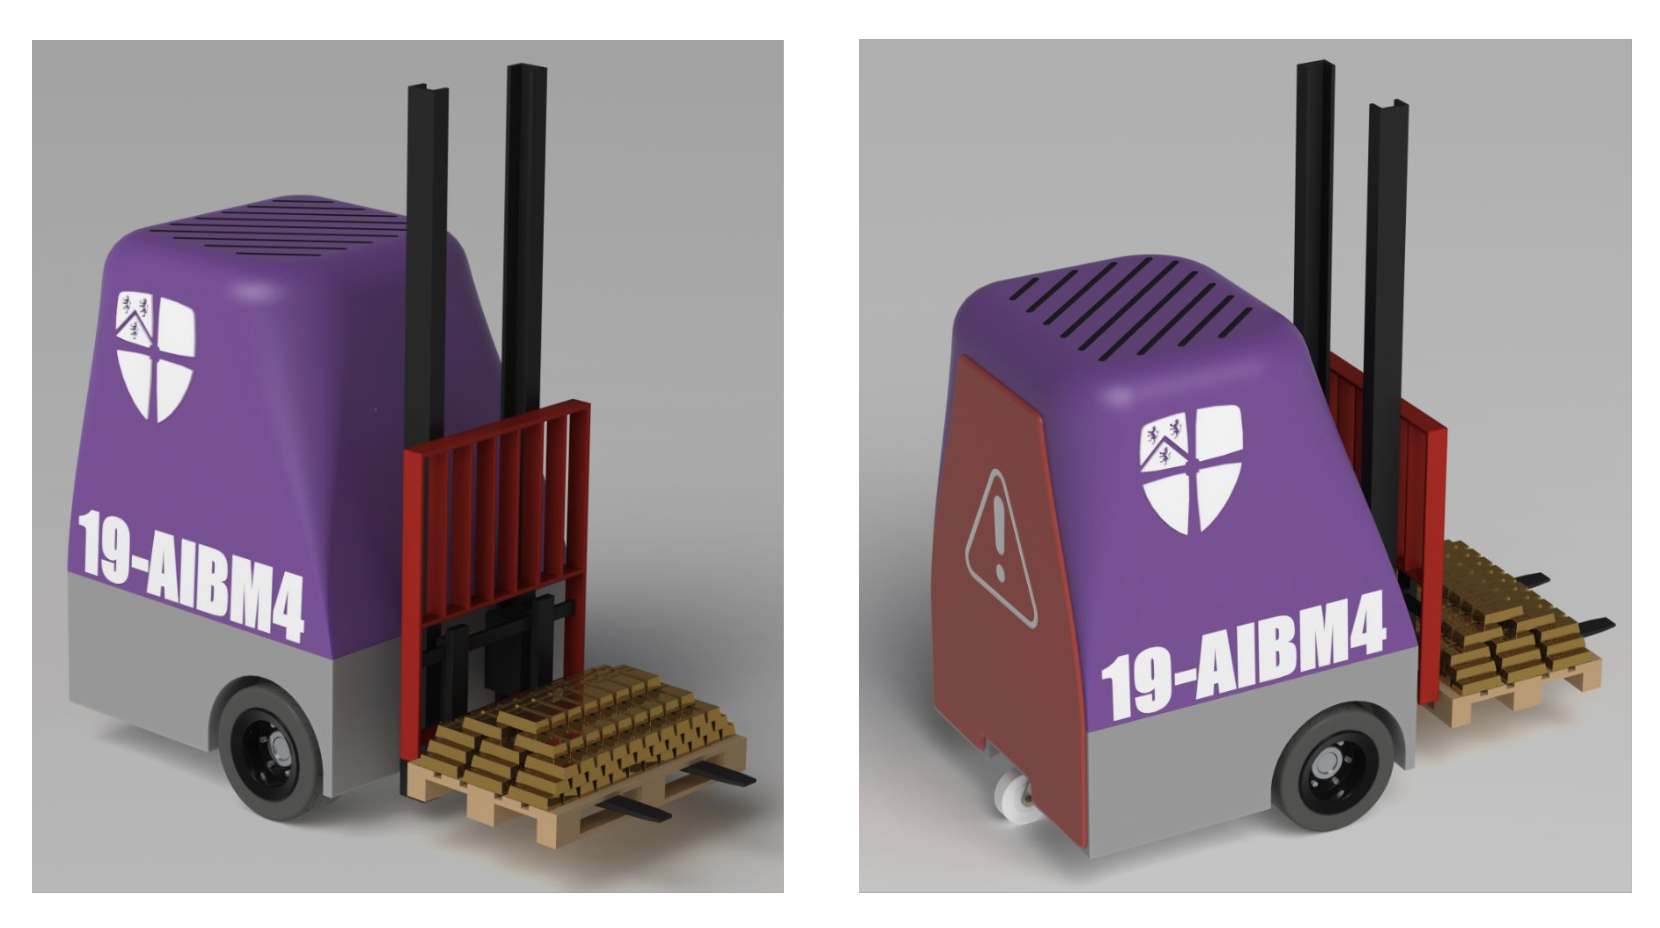
\includegraphics[width=0.65\textwidth]{finaldesign.png}
 %         \label{fig:final design}
%\end{figure}

\newpage

% -------------------------------------------------------------
% MAIN CONTENT
% -------------------------------------------------------------


% -------------------------------------------------------------
% 2. Introduction and Project Scope
% -------------------------------------------------------------
\section{Executive Summary}
This feasibility report looks into the development of an Automated Material Mover (AIBM4), which aims to transport materials autonomously within a factory environment. This would eliminate the need for manual handling of goods, improve productivity and ensure a safer and more sustainable working environment. 
\par Through an iterative design process, we chose a three-wheeled automated forklift design that integrates differential steering around a central axle for maximum manoeuvrability and tape sensing technology for precise movement within a factory environment. To make this design contemporary and sustainable, the body and forks will be made out of steel due to its high reconcilability, while the castor wheel will be made from a pre-consumer nylon, and we will use airless tyres to improve durability and reduce waste.
\par Engineering calculations validate are designs structural integrity and feasibility as well as ensuring compliance with ISO 3691-4  standards. An in-depth cost analysis demonstrates that this automated guided vehicles (AGVs) are financially viable over conventional manual forklifts, due to significant savings in labour and operating costs over time. A break even analysis determines that only 39 units need to be sold to generate a profit, with over 1.4 million forklifts\cite{Statista} being sold worldwide in 2022 year and sales increasing year on year this is very achievable.
\par An adaptable factory layout design has been included which has been optimised for AGV operation, however the material mover has been designed to fit into the majority of modern-day factories. We have also conducted a risk assessment to mitigate any risks as well as created a Gantt chart which to determine that the design process will be finished by the end of March 2025.
\par This report demonstrates the technical, economic and environmental upper hand that an automated material mover can be provide in a modern factory setting.

\section{Introduction}
\subsection{What is the problem that we are attempting to solve?}
Efficient material handling is essential in modern manufacturing, but conventional forklifts still require manual operation. This project seeks to eliminate manual dependency by designing an autonomous material mover.
 
\subsection{Issues with Conventional Manual Material Handling}

Manual labour and forklifts have several key issues within factory environments:

\begin{itemize}
    \item \textbf{Inefficiency:} Human workers require regular breaks, reducing productivity
    \item \textbf{Safety concerns:} Human error can lead to an increased likelihood of an accident as well as a higher chance of injuries.
    \item \textbf{Cost:} Cost of labour is very large, and multiple shifts necessitates additional hiring costs.
    \item \textbf{Reliability:} Human error can lead to materials being moved to the wrong locations.
\end{itemize}

Overall, these issues reduce productivity and compromise workplace safety.



\begin{figure}[htbp]
\section{Project Scope}
    \centering
     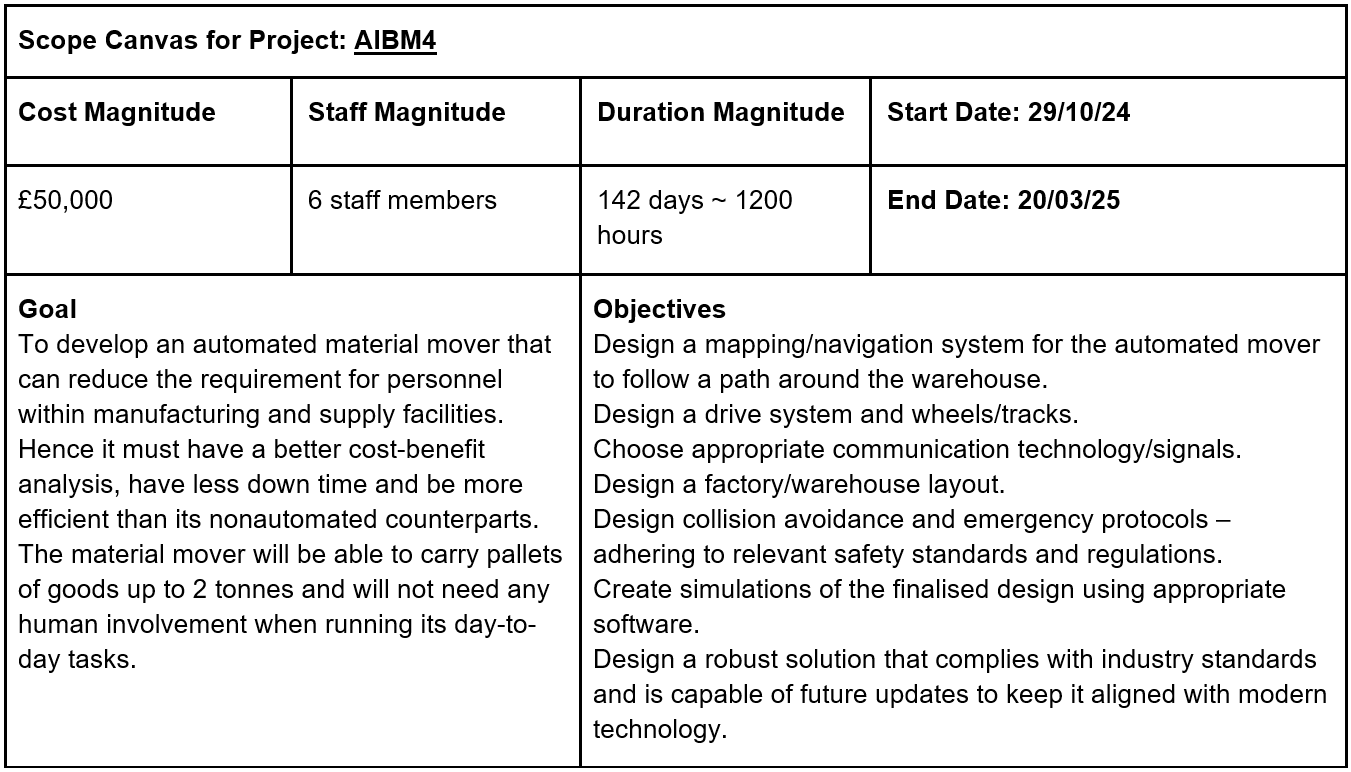
\includegraphics[width=0.9\textwidth]{Scope Canvas 1.png}
     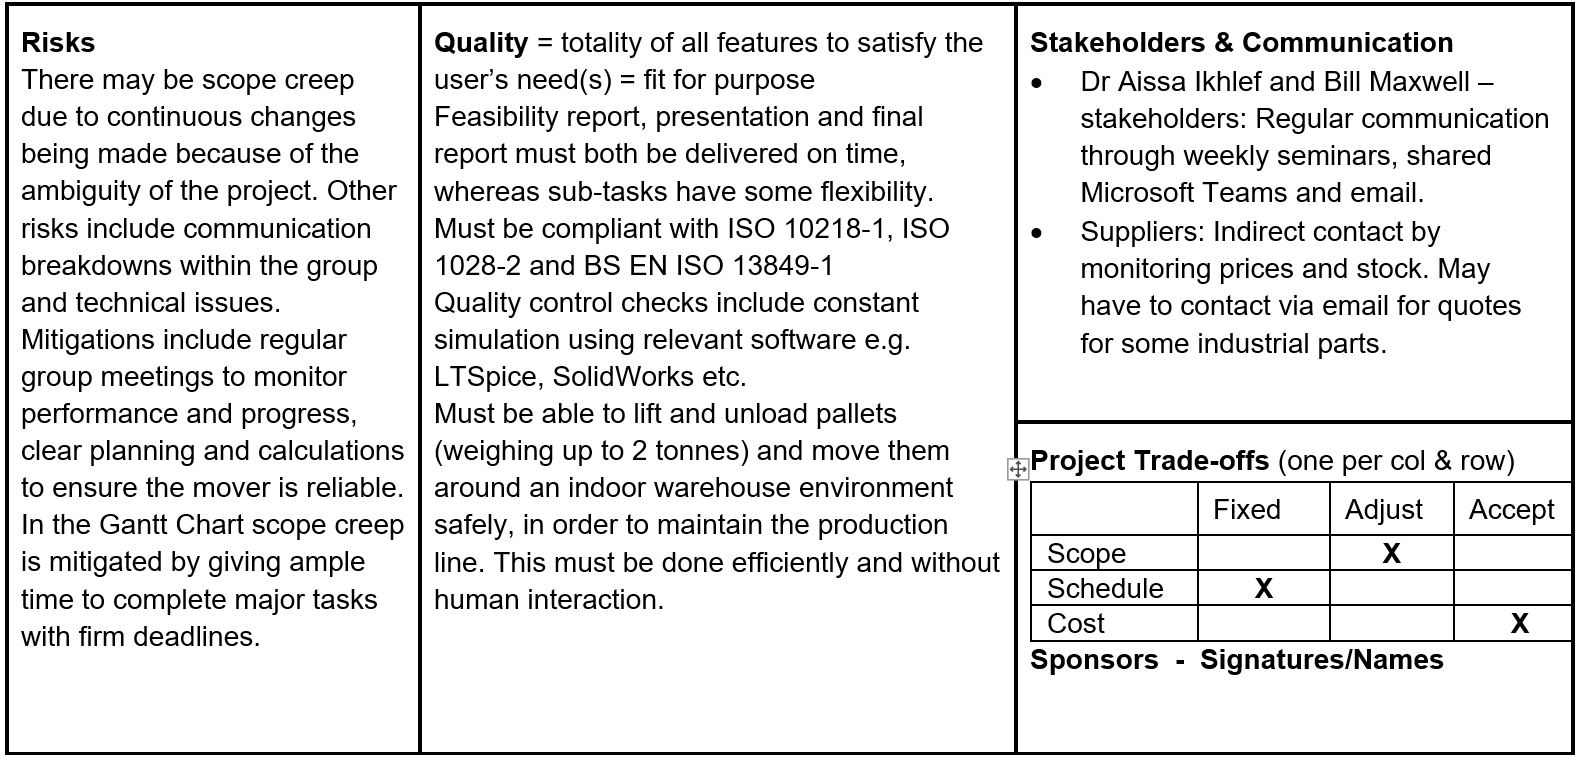
\includegraphics[width=0.9\textwidth]{Scope Canvas 2.png}
     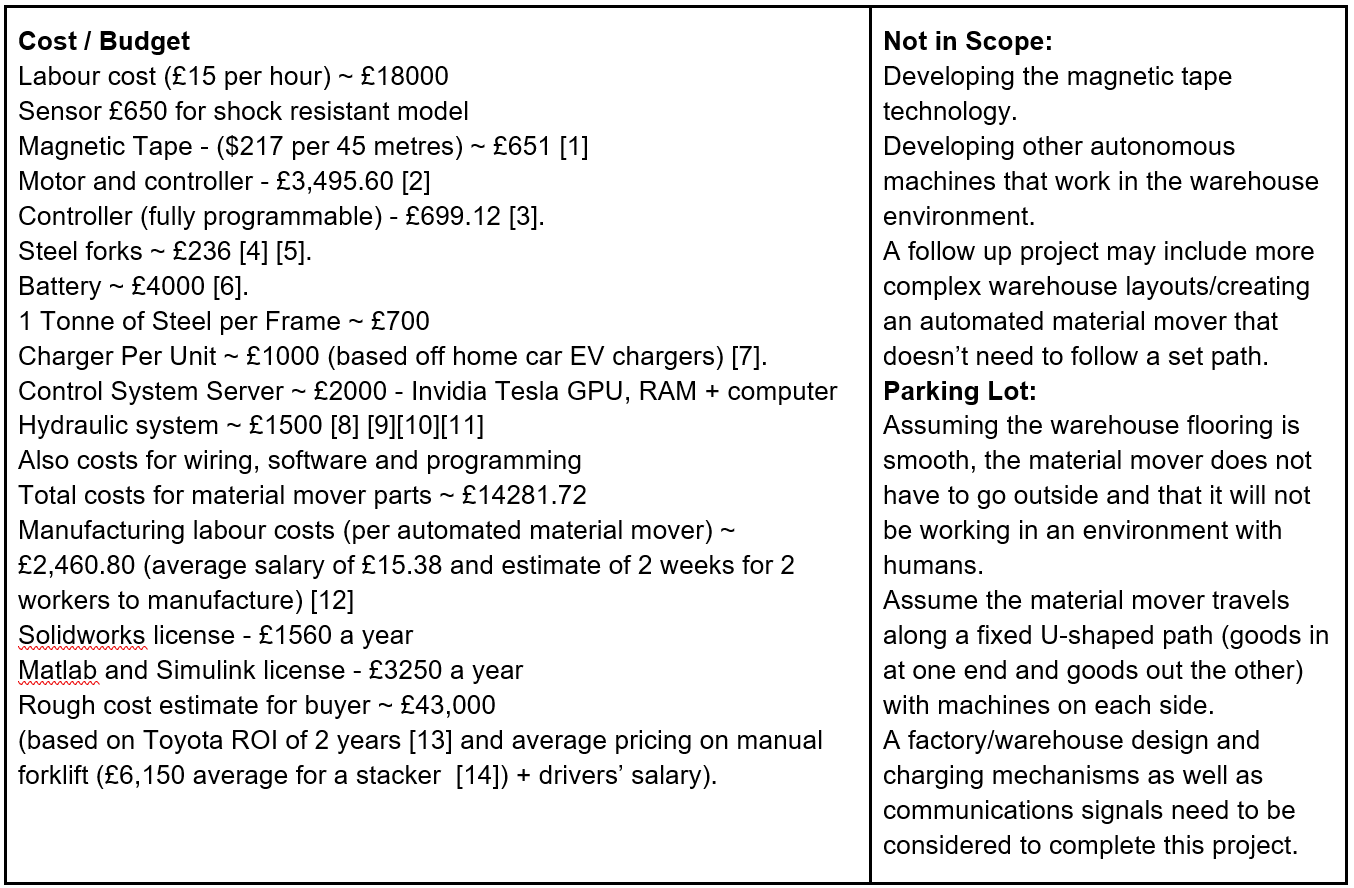
\includegraphics[width=0.9\textwidth]{Scope Canvas 3.png}
   

\end{figure}
\clearpage
\begin{figure}[htbp]

    \centering
     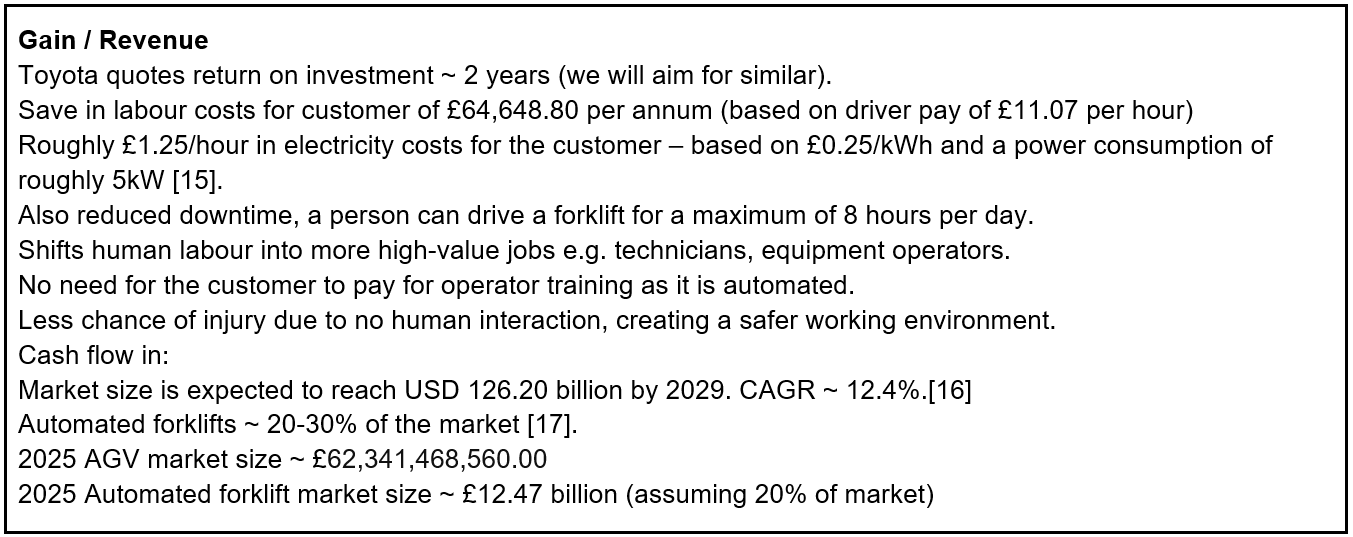
\includegraphics[width=1\textwidth]{Scope Canvas 4.png}
\end{figure}
\FloatBarrier




\begin{figure}[ht]
 
\section{User Requirement Specification (URS)}
    \centering
     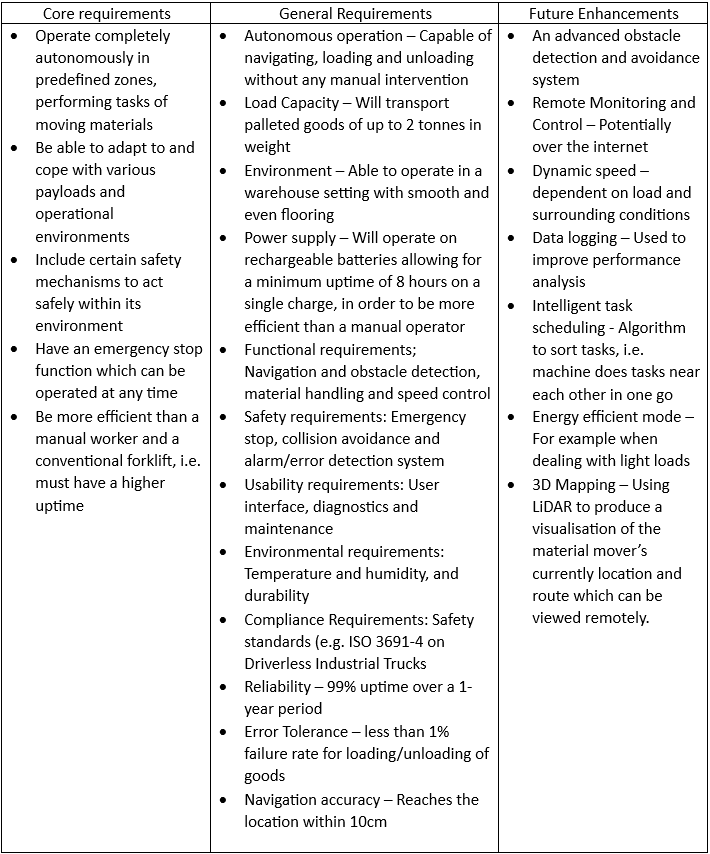
\includegraphics[width=1.05\textwidth]{URS.png}
     \caption{URS – Automated Material Mover Project}
    \label{fig:URS}
\end{figure}
\FloatBarrier

\newpage
% -------------------------------------------------------------
% 3. Concepts
% -------------------------------------------------------------
\section{Concepts}
\subsection{Possible Concepts}
 
\begin{enumerate}
    \item A three-wheeled mover with magnetic tape sensors. This design utilises a compact three wheeled configuration to allow for maximum manoeuvrability in tight spaces. Due to its magnetic tape sensing technology it can accurately navigate predefined paths within a factory setting.
    \item A four-wheeled mover on a monorail. This design uses a monorail to ensure extremely precise movement as well as a four wheel base which makes it very sturdy for lifting goods and transporting them quickly and efficiently.  
    \item A six-wheeled mover with line-following sensors. Six wheels allows for superior stability and load-bearing capabilities. It would use differential steering for its central axis, with the other four wheels being caster wheels, to allow it to spin on the spot making it highly manoeuvrable and versatile.
 \end{enumerate}

\begin{figure}[h!]
    \centering
    % First image and its caption
    \begin{minipage}{0.32\textwidth}
        \centering
        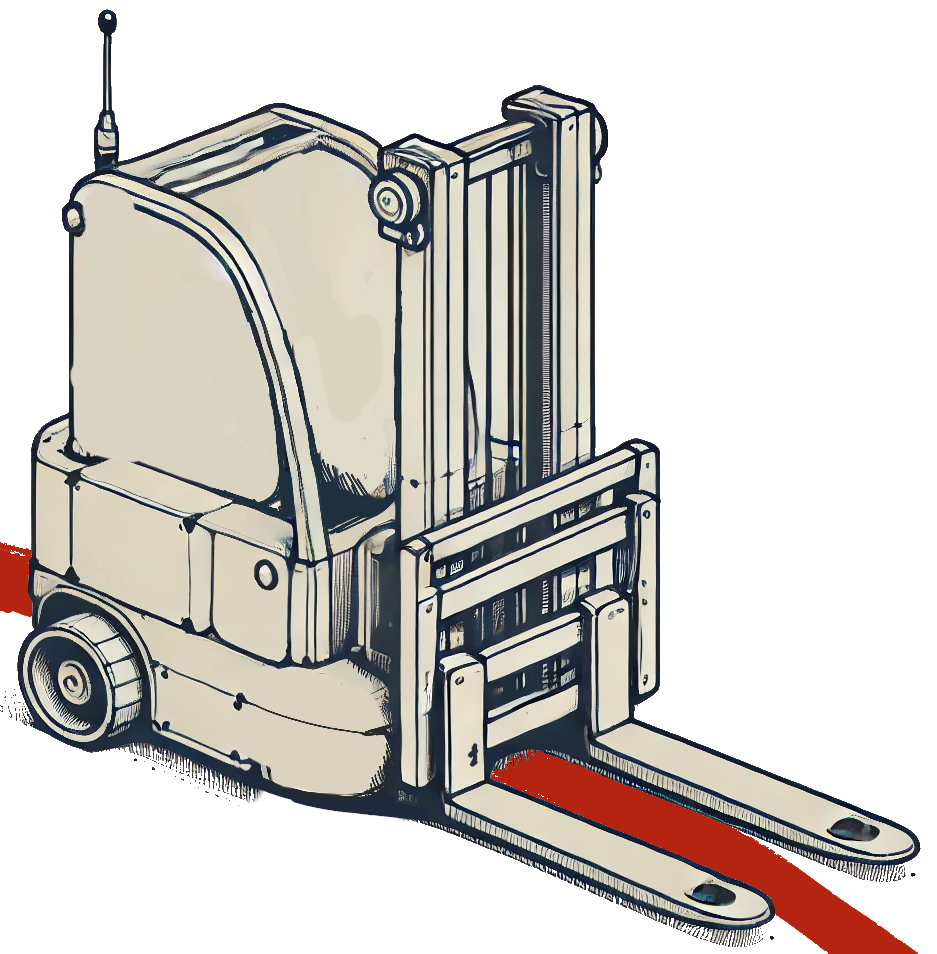
\includegraphics[width=\textwidth]{Simple_sketch_of_an_automated_forklift_robot_with_two_wheels_at_the_back_and_one_wheel_in_the_front.png}
    \end{minipage}%
    \hspace{0.01\textwidth}
    % Second image and its caption
    \begin{minipage}{0.32\textwidth}
        \centering
        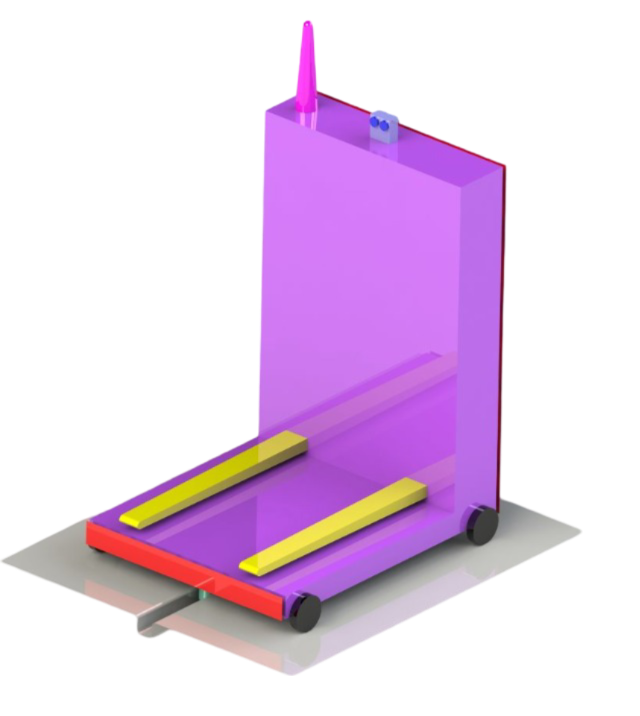
\includegraphics[width=\textwidth]{anna&will's design (1).png}
    \end{minipage}%
    \hspace{0.01\textwidth}
    % Third image and its caption
    \begin{minipage}{0.32\textwidth}
        \centering
        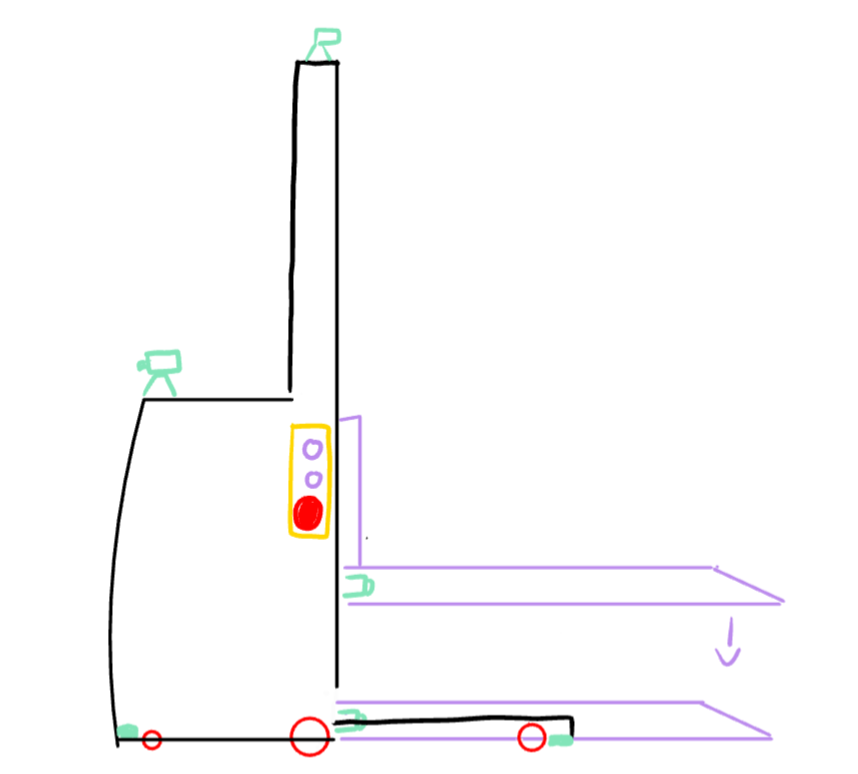
\includegraphics[width=\textwidth]{Louis' design without text.png}
    \end{minipage}
    \hspace{0.01\textwidth}
    
    % Captions below images
    \vspace{0.5mm}  % Adds space between the images and captions
    \begin{minipage}{0.32\textwidth}
        \centering
        \textbf{}Figure 2: Three wheel magnetic tape following design
    \end{minipage}%
    \begin{minipage}{0.32\textwidth}
        \centering
        \textbf{}Figure 3: Four wheel monorail design
    \end{minipage}%
    \begin{minipage}{0.32\textwidth}
        \centering
        \textbf{}Figure 4: Six wheel line following design %%  better to use   \caption{Final design} for automation :D   \label{fig:final_design}
    \end{minipage}
\end{figure}
 

\subsection{Strengths and Weaknesses}
Each concept was evaluated against the URS using a design decision matrix. A summary of this is provided in Table \ref{tab:concept_evaluation} below.


\begin{table}[h!]
\centering
\caption{Concept Evaluation Matrix}
\begin{tabular}{@{}lccc@{}}
\toprule
\textbf{Criteria}      & \textbf{Concept 1} & \textbf{Concept 2} &\hl{\textbf{Concept 3}} \\ \midrule
Load Capacity          & High               & Medium              & Medium            \\
Navigation Efficiency  & Medium             & High                & High              \\
Cost                   & Low                & Medium              & Medium            \\
Ease of Maintenance    & High               & Low                 & Low               \\ \bottomrule
\end{tabular}
\label{tab:concept_evaluation}
\end{table}
\FloatBarrier

% -------------------------------------------------------------
% 4. Chosen Solution
% ------------------------------------------------------------
\section{Chosen Solution}
\begin{figure}[H]
    \centering
    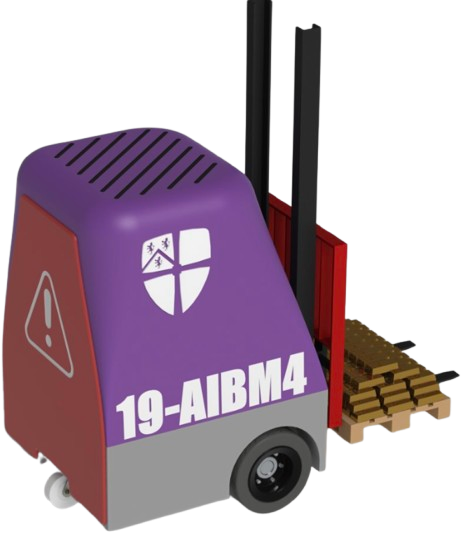
\includegraphics[width=0.4\linewidth]{finaldesign1rb.png}  % Adjusted to 30% of the line width
    \caption{Final design}
    \label{fig:x}
\end{figure}



The initial design that was chosen was Concept one, with some changes to improve performance. For greater manoeuvrability, a counterweight design was chosen, removing the frontmost wheels to allow the lifter to rotate about it's centre.
In order to improve sustainability, the body and forks are likely to be made from steel because it has the highest recycling rate among all materials used in construction and engineering \cite{baker2023}. The castor wheels can be made of high-quality pre-consumer nylon (from the waste of polyester production) \cite{eco2022} and the drive wheels can be airless tires, as it reduces the amount of rubber that goes into landfills and improves fuel efficiency \cite{ImperialTyres}.

\subsection {Stress and Deflection Calculations}
Assuming the fork is a beam of uniform cross section fixed at the left end to the forklift, it can be modelled as shown in {figure 6}.
\begin{figure} [H]
    \centering
    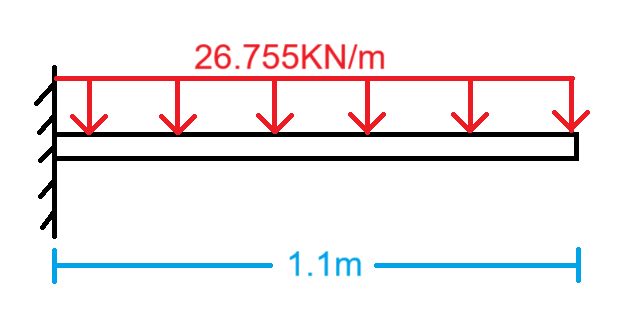
\includegraphics[width=0.5\linewidth]{fork as a beam diagram.png}
    \caption{Diagram showing the force diagram of a singular fork.}
    \label{fig:x}
\end{figure}
This is using a factor of safety of three for the maximum load, as specified by ISO-2330 for the prototyping of forklift forks. (INSERT REFERENCE)
Thus using Macauley's method the equation for deflection of a steel-203 fork with E = 190GPa (INSERT REFERENCE), height (h) = 40mm and width (b) =100mm (INSERT REFERENCE) is given by:
\begin{equation}
   \nu = \frac{3}{304000} \left( \frac{-16186.5}{2}x^2 + \frac{29430}{6}x^3 - \frac{26755}{24}x^4 \right)
\end{equation}
Therefore maximum deflection is at \(x = 1.1 \, \text{m}\), which is \(\nu = -4.83 \, \text{cm}\).
For fatigue, following ISO-2330 standards a cyclic stress amplitude of 1.655MPa was obtained using equation (2).
\begin{equation}
   \text{Cyclic Stress Amplitude} = \left (\frac{Force}{Area} \right)
\end{equation}
The obtained value is smaller than the minimum fatigue limit of \(175 \text{MPa}\) so no cracking due to fatigue will occur.
\subsection{Centre of Mass calculations}
In a counterbalance forklift design, the centre of mass is kept between the front and rear wheels through a large counterbalance positioned far back. Normally the mass of the battery contributes to this. In order to determine whether a design  is  safe from tipping, several calculations must be performed.
\begin{figure} [H]
    \centering
    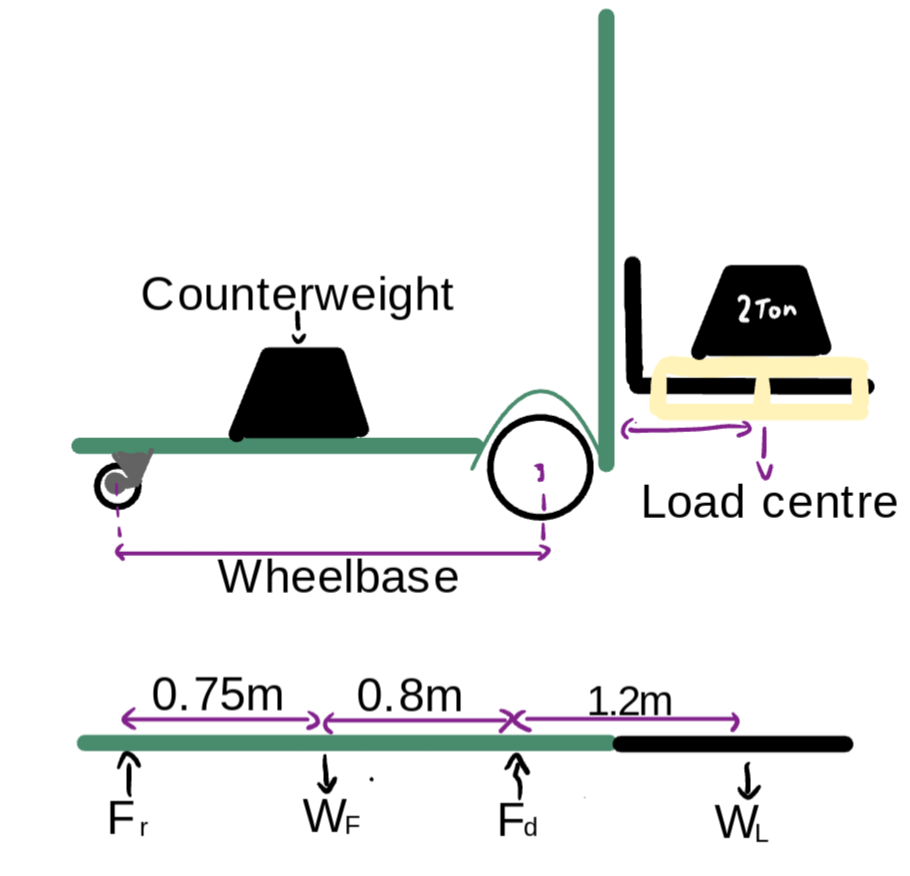
\includegraphics[width=0.5\linewidth]{Tipping Calculations.png}
    \caption{Diagram showing mass distribution in a counterbalance forklift, and free body diagram of the same}
    
\end{figure}
\subsection{Expected Cost}

{The estimated cost of the product \cite{P. Hinz} is £60,000, and this covers:}
\begin{itemize}
    \item All the hardware for the autonomous material mover 
    \item All of the software acquisition and development for navigation, obstacle detection, and task automation.
    \item The implementation of the system into a conventional factory; however, this will likely differ on a site-to-site basis.
\end{itemize}

\begin{table}[h!]
    \centering
    \begin{tabular}{|l|r|}
        \hline
        \textbf{Cost Item}          & \textbf{Amount (£)} \\ \hline
        Labour Costs                 & 18,000.00           \\ \hline
        Material Costs              & 15,099.12           \\ \hline
        Overheads                   & 10,000.00           \\ \hline
        Software and Simulation     & 2,000.00            \\ \hline
        Contingency                 & 4,900.88            \\ \hline
        \textbf{Total Estimated Cost} & \textbf{60,000.00}  \\ \hline
    \end{tabular}
    \caption{Breakdown of Expected Costs for the Autonomous Material Mover}
    \label{tab:expected_costs}
\end{table}

\begin{figure}[ht]
    \centering
    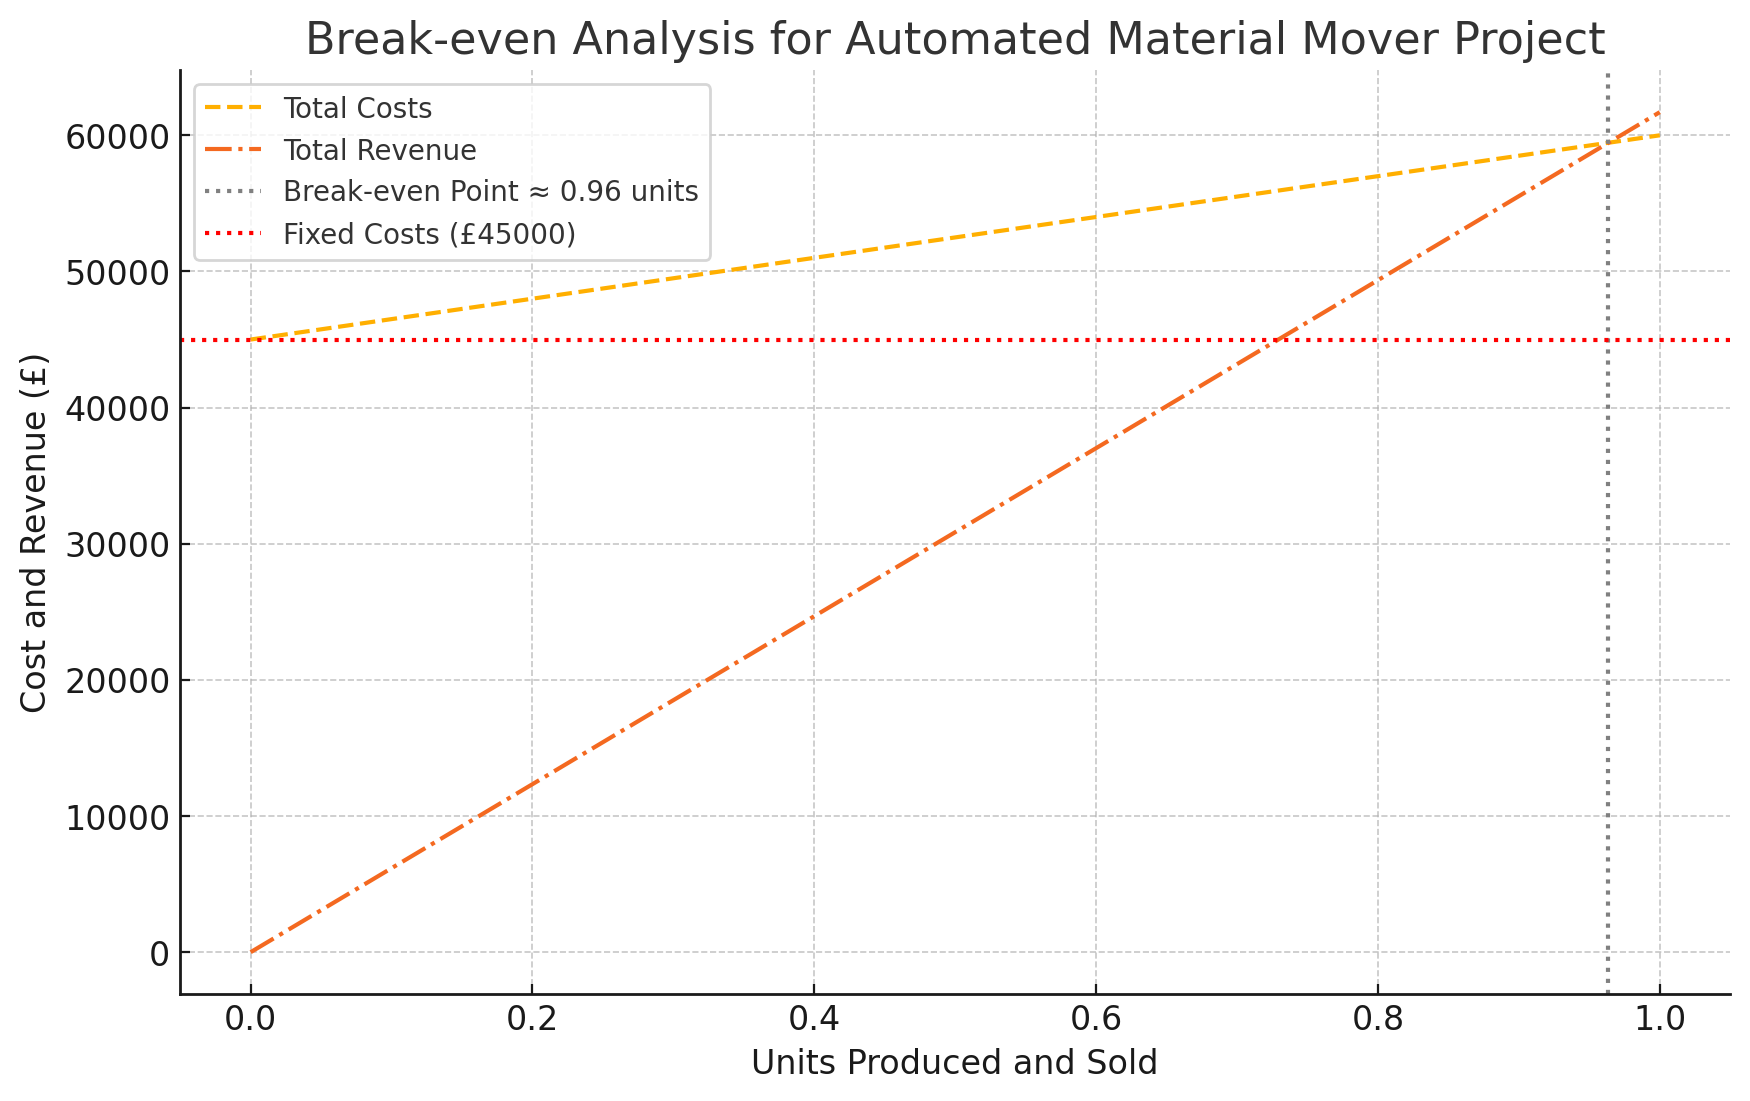
\includegraphics[width=1\textwidth]{breakeven.png}  % Adjust width as needed
    \caption{Breakeven Point Analysis}
    \label{fig:breakeven}
\end{figure} 

\FloatBarrier
\subsection{Cost Comparison for a Customer}
Whilst this product may seem expensive at first to potential customers, it has distinct financial and logistical advantages over manual forklifts. A 2-ton manual stacker truck can cost anywhere from £8000 for a standing operator push model, to over £25000 for a counterbalance truck. In addition to the cost of the stacker there is the cost of paying operators. 
This soon adds up, with hourly minimum wage in the UK being £11.44, this being the largest factor in running costs. An automated stacker eliminates this expense, whilst also being able to work continuously with only breaks for charging.

It should be considered that automated forklifts do on average move slower than regular manually driven forklifts. This means that it takes around 1.3-1.5 automated forklifts to do the same work as a single manned truck \cite{Pastor-Tella2024}. 
Taking these things into consideration, the following table assumes a factory using two manned forklifts, and how these costs would compare to three AGVs.
 

\begin{figure}[h!]
    \centering
     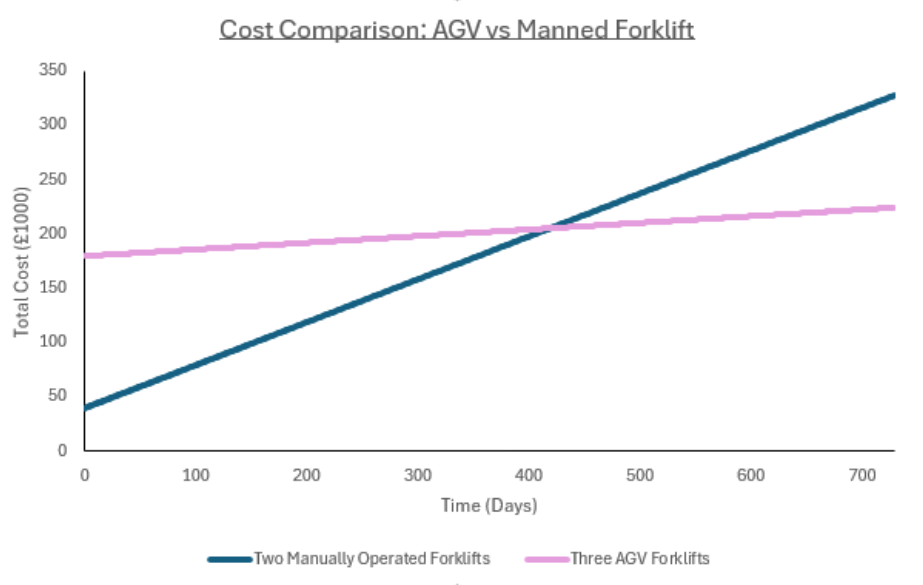
\includegraphics[width=0.75\textwidth]{CostComparisonGraphUpdatedV2.png}
        \caption{Cost Comparison: AGVs vs Manned Forklifts}
         \label{fig:timeline}
\end{figure}
\FloatBarrier
Cost per unit taken as £60,000 for an AGV, compared with £20,000 for a manual forklift. From the graph we can see that after 420 days of operation the three AGV forklifts become more economical in comparison to the two manually operated forklifts. The full cost comparison information is shown in Table 3.



\begin{table}[htbp]
\centering
\begin{tabular}{|l|l|l|}
\hline
\textbf{Cost Factor}                   & \textbf{Manual Forklifts}           & \textbf{AGVs } \\ \hline
\textbf{Initial Cost per Unit}          & £20,000                             & £60,000                               \\ \hline
\textbf{Number of Units}                & 2                                    & 3                                     \\ \hline
\textbf{Total Initial Cost}             & 2 × £20,000 = £40,000               & £180,000                \\ \hline
\textbf{Annual labour cost per forklift }& £11.44× 16×365 = £66,810      & £0                                    \\ \hline
\textbf{Total Annual Labor Cost (16 hours a day)}        & 2 x £66,810 = £129,297.6    & £0                                    \\ \hline
 \textbf{Electricity cost per year (25.46p per kWh) } & £14,868&£22,302\\\hline  
 
\textbf{Total Annual Operating Cost}    & £148,487& £22,302\\ \hline
 
  
\end{tabular}

\caption{Cost Breakdown for Manual and Automated Forklifts}
\end{table}


 


\FloatBarrier
\begin{figure}[ht]
\subsection{Factory layout }
\centering
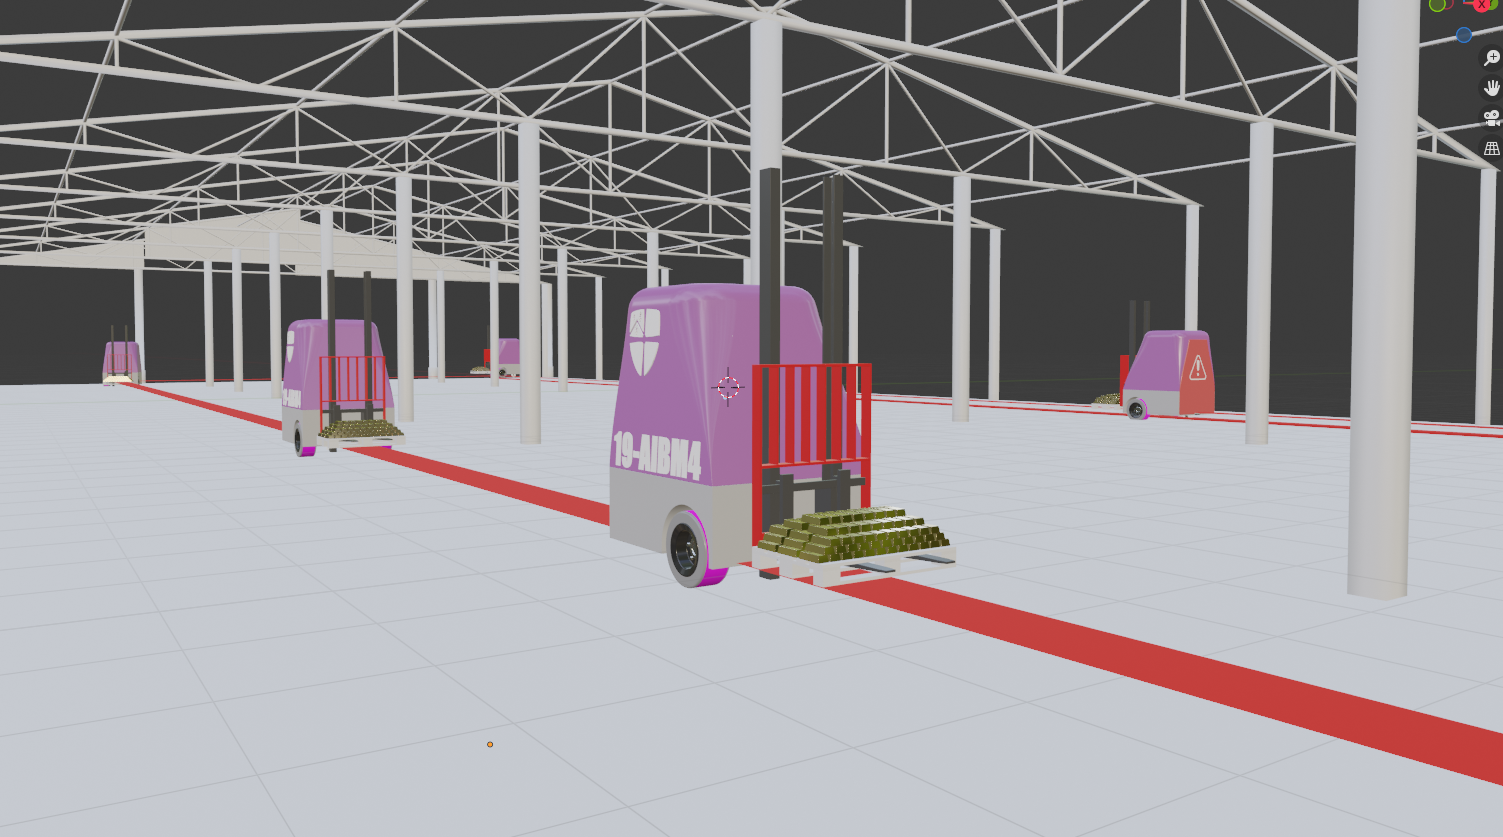
\includegraphics[width=1\linewidth]{factory layout1.png}
\caption{Factory design layout}
\label{fig:factory_layout}
\end{figure}

\begin{figure}[ht]
    \centering
    \begin{minipage}{0.45\linewidth}
        \centering
        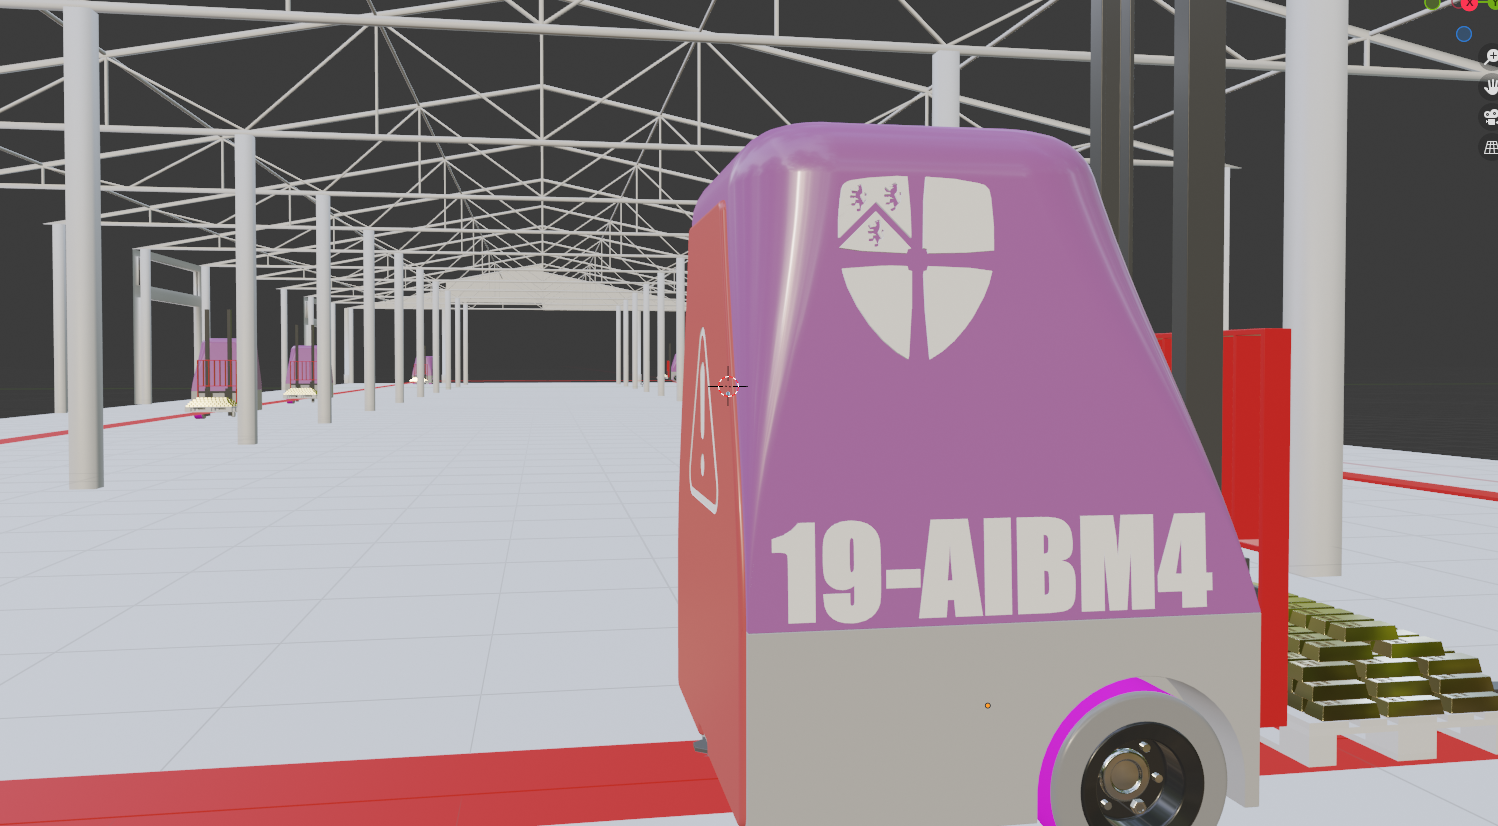
\includegraphics[width=\linewidth]{blender_animation.png} % Replace with your Blender animation image
        \caption{Blender Animation}
        \label{fig:blender_animation}
    \end{minipage}
    \hspace{0.05\linewidth}
    \begin{minipage}{0.45\linewidth}
        \centering
        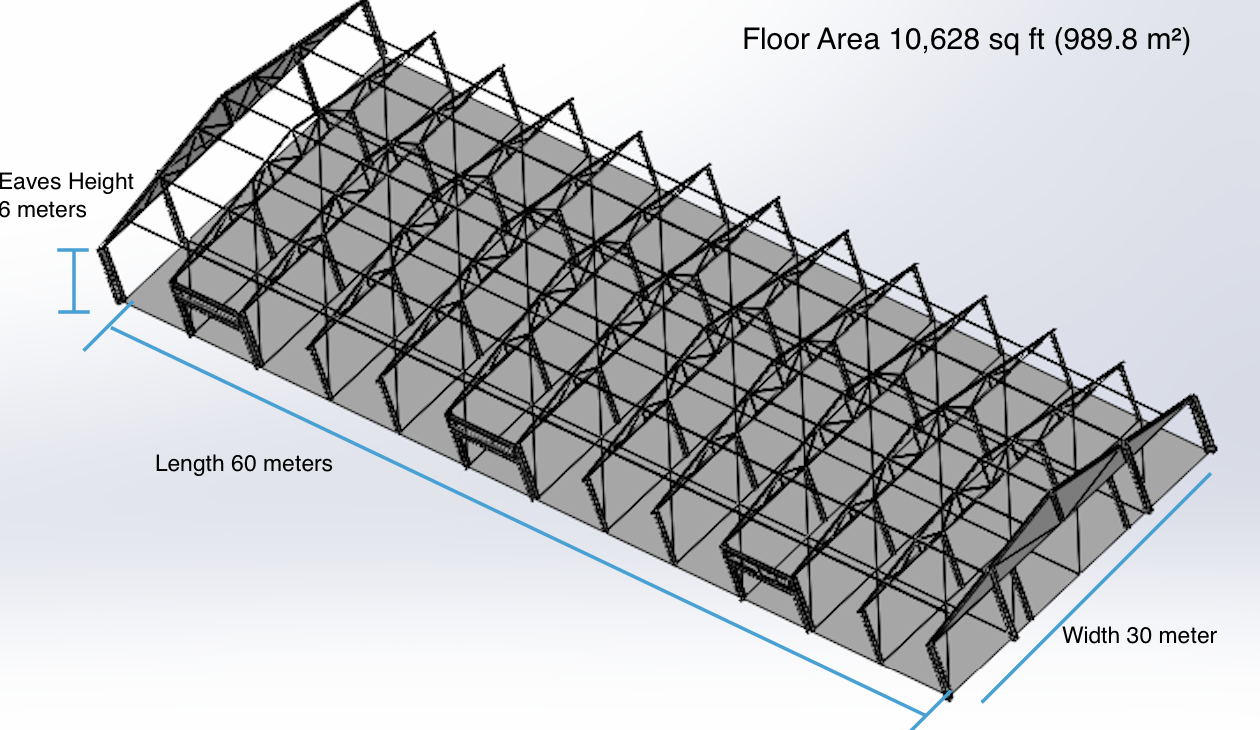
\includegraphics[width=\linewidth]{factory layout dimension.png}
        \caption{Factory design layout}
        \label{fig:factory_layout}
    \end{minipage}
\end{figure}

 


Based on the information from the EG Propertylink listing for Unit 5, Hurworth Road, Aycliffe Business Park \cite{mileway_hurworth_2024}, the CAD factory layout design integrates the key features and constraints of the property.  Line-following forklifts rely on predefined paths marked by visible or magnetic lines (often in the form of tape or sensors) on the floor. The layout was optimized to include narrower aisles suitable for line-following AGVs,  ensuring they have sufficient room to follow the lines without obstruction which take full advantage of the 6-meter eaves height.

Clearly defined line-following paths throughout the facility marked with high-visibility lines (magnetic strips), guide the forklifts through the warehouse, directing them to storage zones, picking locations, and loading bays. A dedicated area for charging stations was incorporated into the layout . Automated docking stations were strategically located near the production and storage zones, ensuring AGVs can easily return to their charging points without disrupting material handling operations. 

 

 
\begin{figure}[h!]
 \section{Risk assessment }
    \centering
    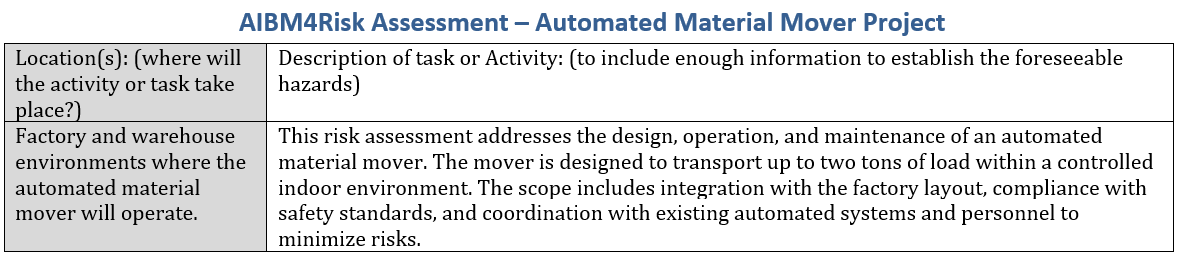
\includegraphics[width=0.85\textwidth]{Risk1.png}
    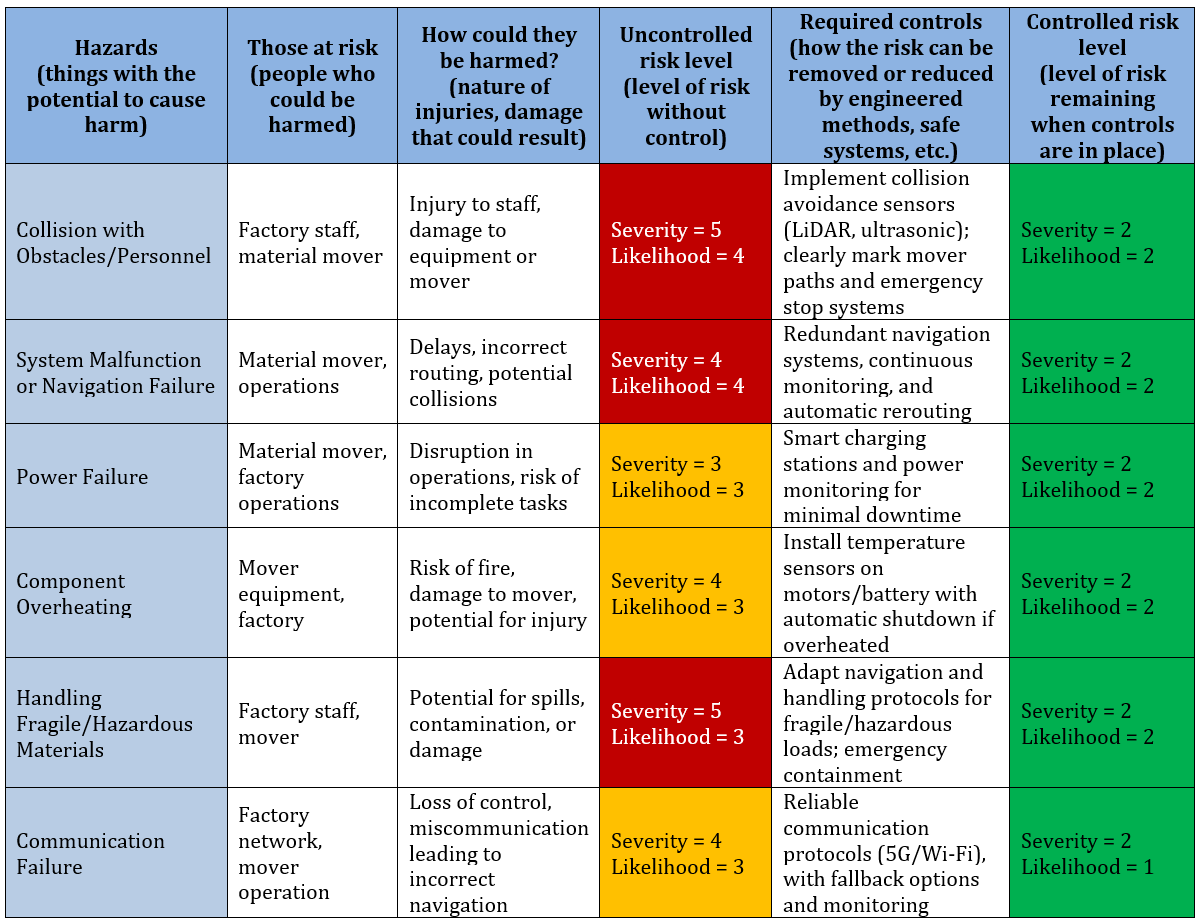
\includegraphics[width=0.85\textwidth]{Risk2.png}
    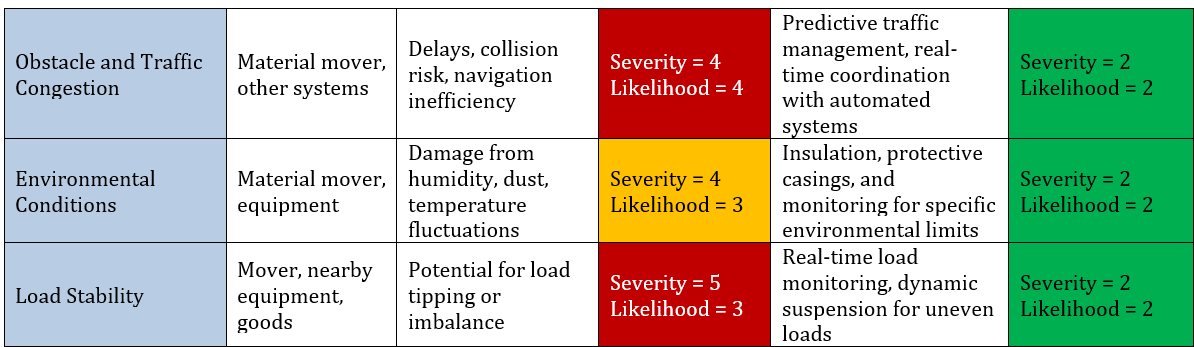
\includegraphics[width=0.85\textwidth]{Risk3.png}
    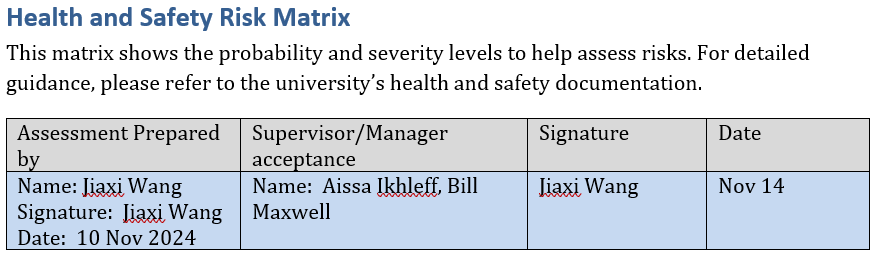
\includegraphics[width=0.85\textwidth]{Risk4.png}
    \caption{Risk Assessment – Automated Material Mover Project}
    \label{fig:risk_assessment}
\end{figure}
\FloatBarrier

 

% -------------------------------------------------------------
% 6. Project Schedule
% -------------------------------------------------------------
\section{Project Schedule}

In order to plan out the schedule throughout the project, a Gantt Chart was created to plan out the hours worked every week, ensuring no tasks are ignored or missed out, giving them ample time to be completed. Additionally, leaving contingency hours caters for scope creep and any drastic changes that need to be made and also giving flexibility to change tasks and the hours put into them. The dynamic Gantt Chart in  figure \ref{fig:x}, made using Microsoft Excel, shows how complete each task is, and helps to visualise which tasks are on track, ahead or behind schedule. 
\begin{figure}[h!]
 \subsection{Gantt Chart}
    \includegraphics[width=1\textwidth]{BIGGER Gantt chart.png}
    \caption{Dynamic Project Gantt Chart}
    \label{fig:x}
\end{figure}

\begin{figure}
    \centering
    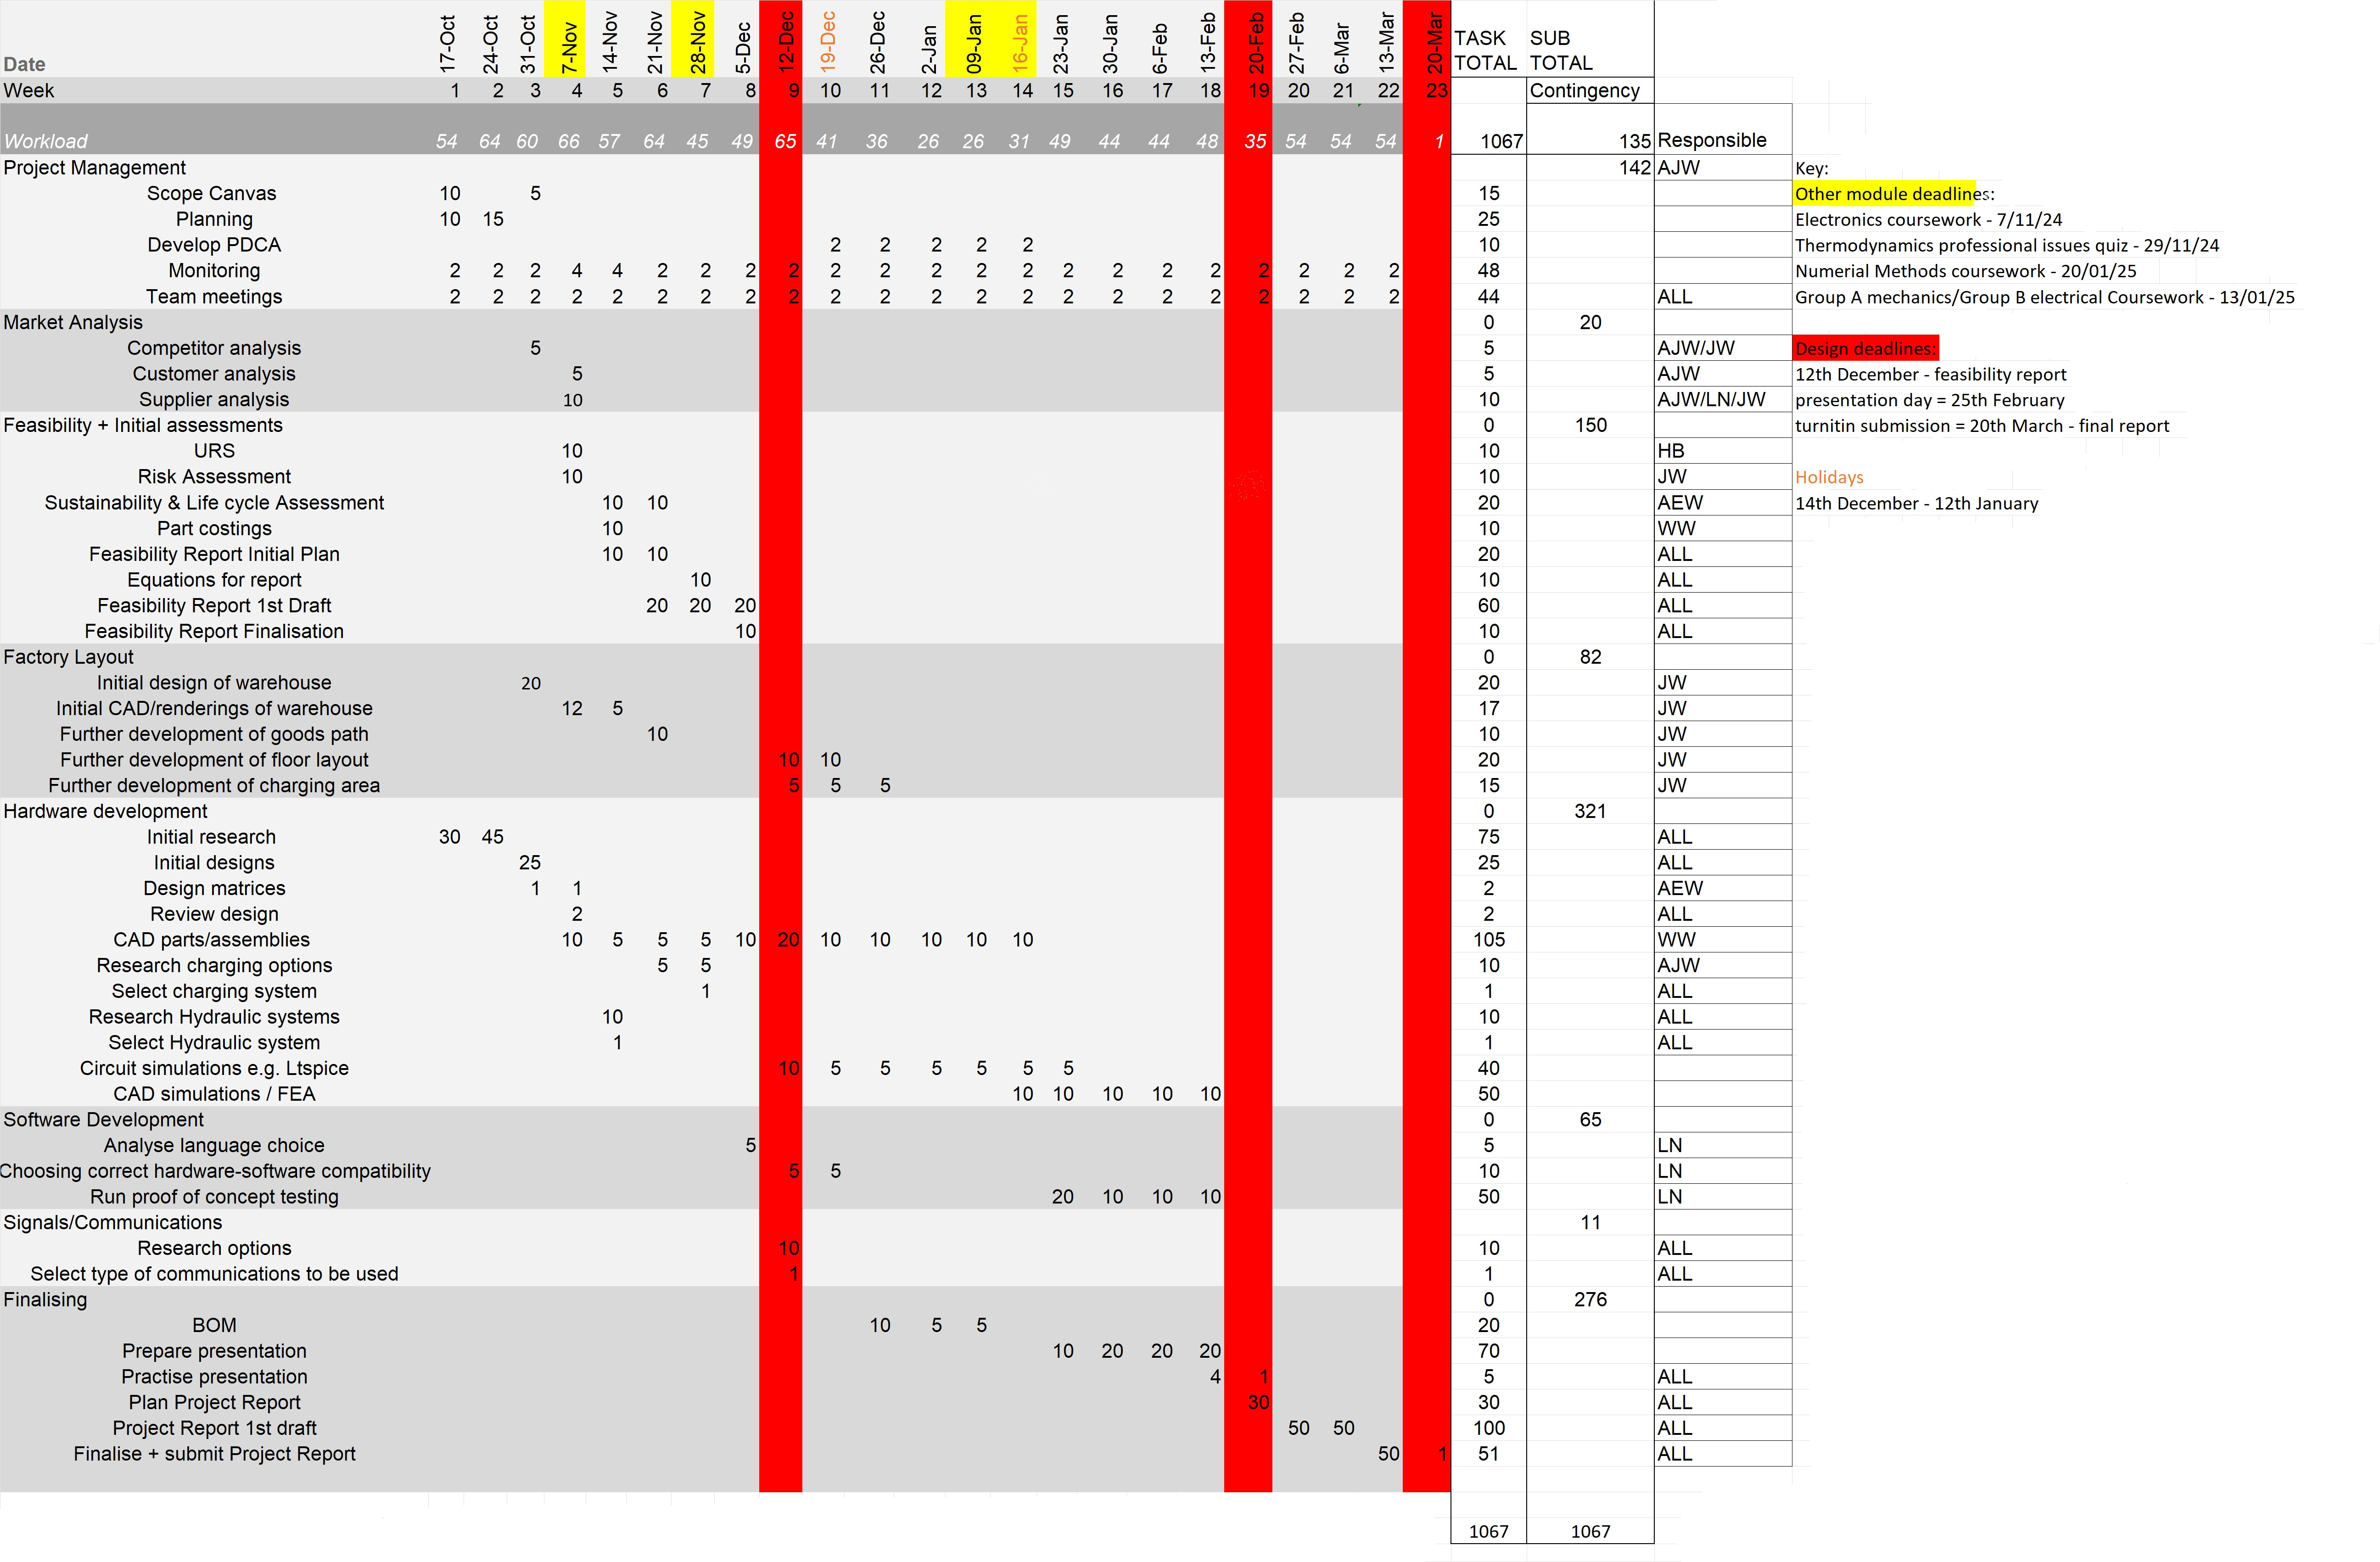
\includegraphics[width=1\linewidth]{Gantt plan final.jpg}
    \caption{Planning Gantt Chart}
    \label{fig:y}
\end{figure}
The planning Gantt Chart, figure \ref{fig:y}, showcases the weekly hours expected to be put into tasks and helps to ensure a balanced workload throughout the project. It also allows foresight for deadlines and other departmental commitments so that the workload can be planned around these accordingly. The majority of first term was planned around choosing a feasible design for the material mover and the research and drawings for this, as well as the factory layout the mover would work in. This provides a strong basis for the remainder of the project which focuses on CAD, software proof of concept and other simulations. This plan also allows for scope creep, having 135 contingency hours, and so means the project has ample time to be complete. 

\begin{figure}[h!]
 \subsection{Meeting Minutes}
    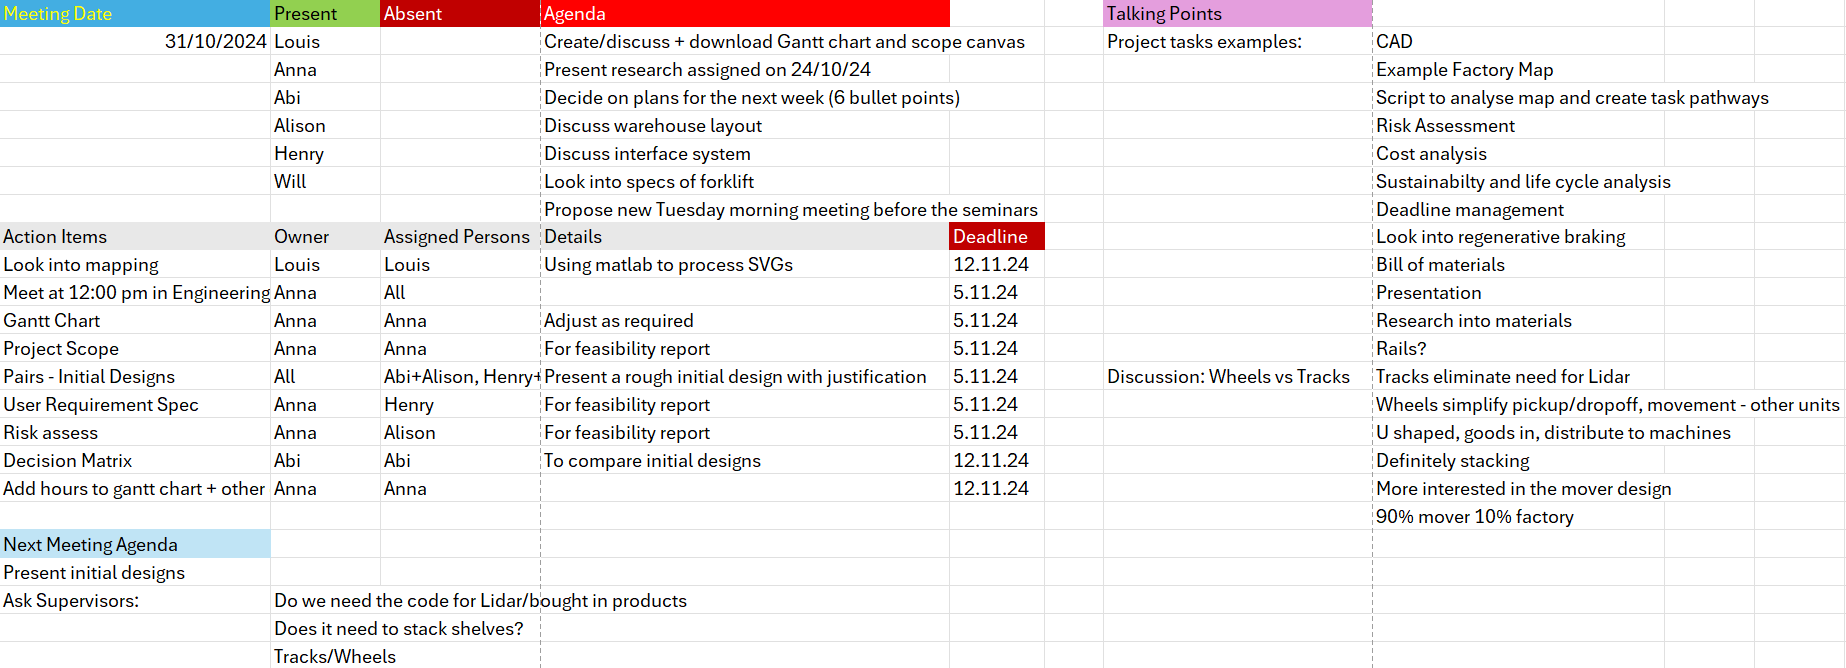
\includegraphics[width=1\textwidth]{HalloweenMinutes1.png}
    \caption{Meeting minutes from 31/10/24}
    \label{fig:x}
\end{figure}
  
Meeting minutes are a core component for the project management of this process. They are a detailed record of all discussions, decisions and assigned tasks. They are taken by the secretary every meeting, which is at least biweekly ensuring consistent and efficient collaboration. This ensures that all topics of discussion are covered and that appropriate tasks are assigned regularly. Maintaining detailed minutes ensured that the whole team was aligned on priorities and deadlines as well as holding people accountable and reducing the risk of miscommunication.

\begin{thebibliography}{99}
\footnotesize

\bibitem{Statista}
Statista, "Global forklift truck market volume from 2018 to 2022"
\textit{https://www.statista.com/}
Avaliable at:
https://www.statista.com/statistics/1451892/global-forklift-truck-market-volume
(accessed Dec. 05, 2024)
\bibitem{MathWorks}
MathWorks, “What Is SLAM (Simultaneous Localization and Mapping) – MATLAB \& Simulink,” \textit{uk.mathworks.com}.  
Available at: \url{https://uk.mathworks.com/discovery/slam.html} (accessed Nov. 20, 2024).
 

\bibitem{ToyotaForklifts}
Toyota Forklifts, “Automated Warehouse Trucks,” \textit{toyota-forklifts.co.uk}.  
Available at: \url{https://toyota-forklifts.co.uk/automated-solutions/automated-warehouse-trucks/} (accessed Nov. 20, 2024).

\bibitem{Forkify}
Forkify, “Forklift Cost Buyers Guide,” \textit{forkify.com}.  
Available at: \url{https://forkify.com/buyers-guide/forklift-cost/} (accessed Nov. 20, 2024).


\bibitem{LangleyShop}
Langley Shop, “Forklift Forks 100x40x1200 Class 2A,” \textit{langleyshop.co.uk}.  
Available at: \url{https://www.langleyshop.co.uk/product/forklift-forks-100x40x1200-class-2a/} (accessed Nov. 20, 2024).

\bibitem{CheckaTrade}
Checkatrade, “Electric Car Charger Installation Cost,” \textit{checkatrade.com}.  
Available at: \url{https://www.checkatrade.com/blog/cost-guides/electric-car-charger-installation-cost/} (accessed Nov. 20, 2024).

\bibitem{SalaryExpert}
Salary Expert, “Forklift Driver Salary in South Korea,” \textit{salaryexpert.com}.  
Available at: \url{https://www.salaryexpert.com/salary/job/forklift-driver/south-korea?form=MG0AV3} (accessed Nov. 20, 2024).

\bibitem{MordorIntelligence}
Mordor Intelligence, “Automated Material Handling Market,” \textit{mordorintelligence.com}.  
Available at: \url{https://www.mordorintelligence.com/industry-reports/automated-material-handling-market} (accessed Nov. 20, 2024).

\bibitem{GrandViewResearch}
Grand View Research, “Automated Guided Vehicle (AGV) Market,” \textit{grandviewresearch.com}.  
Available at: \url{https://www.grandviewresearch.com/industry-analysis/automated-guided-vehicle-agv-market} (accessed Nov. 20, 2024).

\bibitem{baker2023} T. Baker, ``5 Reason Why Structural Steel is Such a Sustainable Material,'' \textit{Baker Steel Trading}, 2023. [Online]. Available: \url{https://www.bakersteeltrading.co.uk/is-structural-steel-sustainable/}. [Accessed: Nov. 21, 2024].

\bibitem{eco2022} S. Co, ``We use ECO-FRIENDLY production techniques and technology,'' \textit{ENJOYING GO}, Sep. 21, 2022. [Online]. Available: \url{https://www.enjoycaster.com/en/solutions/product/eco-friendly-production}. [Accessed: Nov. 25, 2024].

\bibitem{ImperialTyres} 
``How is the tyre industry becoming more sustainable?,'' \textit{Imperial Tyres}, 2024. [Online]. Available: \url{https://www.imperialtyres.co.uk/blog/how-is-the-tyre-industry-becoming-more-sustainable/}. [Accessed: Nov. 21, 2024]

\bibitem{P. Hinz}
P. Hinz, “How Much Electricity does a Forklift Use per Hour?,” Adaptalift, Sep. 2021. \url{https://www.adaptalift.com.au/blog/how-much-electricity-does-a-forklift-use-per-hour }(accessed Nov. 25, 2024).

 \bibitem{mileway_hurworth_2024}
Mileway, “Hurworth Road, Newton Aycliffe Industrial Estate,” \url{https://mileway.com/properties/gb/portfolio/hurworth-road-newton-aycliffe-industrial-estate/} (accessed Dec. 2, 2024).
 
\bibitem{Pastor-Tella2024}
A. Pastor-Tella, ``AGV Cost Whitepaper,'' \textit{Wiferion}, 2024. Available: \url{https://outlook.office365.com/mail/id/AAQkADQ4MWIzM2EyLWQ1MTUtNGY5Ni04OWJhLWZjZDc0MDM5MTczYQAQAA1BfmZRJjlAknOSshQGypA%3D/sxs/AAMkADQ4MWIzM2EyLWQ1MTUtNGY5Ni04OWJhLWZjZDc0MDM5MTczYQBGAAAAAAA82oxQ1EQrR5h73Xq830VeBwBsJyu3A%2BNJQbAH2RRo67L8AAAAAAEMAABsJyu3A%2BNJQbAH2RRo67L8AAE1CmVAAAABEgAQAIuw1RKsTxlAt6tpt4BAJwE%3D}.




\bibitem{crown2024}

Crown Equipment Corporation, \textit{Achieving Sustained Automated Forklift Performance}, 2024, \url{https://www.crown.com/en-us/blog/articles/automation/Achieving-Sustained-Automated-Forklift-Performance.html#:~:text=Fortunately%2C%20automated%20forklifts%20require%20much,on%20and%20within%20the%20vehicle.} (Accessed: December 2, 2024).


% -------------------------------------------------------------

% -------------------------------------------------------------
% BIBLIOGRAPHY (LOCAL) - Uncomment to use instead of BIB
% ------------------------------------------------------------
 

\end{thebibliography}
 

% Start bibliography
% %                                                             % Can be in a separate file, \input(...)
                      % Author names
%         Plastic deformation of cellular materials,                                  % Title of publication
%         \textit{Reference Module in Materials Science and Materials Engineering},   % Journal name
%         2016.                                                                       % Vol, num, pg, year
% %
% \bibitem{Lee:2017aa} J.H. Lee, D.R. Howel, W.P. Meehan III, G.L. Iverson, A.J. Gardner.
%         Effects of Exercise on Sport Concussion Assessment Tool--Third Edition Performance in Professional Athletes,
%         \textit{The Orthopaedic Journal of Sports Medicine},
%         \textbf{5}(9):1--7, 2017. 
% %
% \bibitem{Lang:1988aa} R.J. Lang.
%         \textit{The complete book of origami: Step-by-step instructions in over 1000 diagrams},
%         Dover Publications, Inc.
%         1988. 
% %
% \bibitem{Kingslake:1992aa} R. Kingslake.
%         \textit{Optics in photography},
%         SPIE Optical engineering press
%         1992. 
% %
% \bibitem{Chen:2011ab} W. Chen, B. Song.
%         \textit{Split Hopkinson (Kolsky) bar: Design, Testing and Applications},
%         Mechanical Engineering Series, Springer
%         2011. 
% %
% \bibitem{Fairlie:2008aa} G.E. Fairlie, R. Hart, E.J. Draper.
%         \textit{Structural response to high explosive blast loading},
%         in MABS 20 - Military Aspects of Blast and Shock,
%         2008. 
% %
                                      % End bibliography

% -------------------------------------------------------------
% LISTS OF FIGURES AND TABLES
% -------------------------------------------------------------
\section{Appendices}
\renewcommand{\listfigurename}{Figures}
\renewcommand{\listtablename}{Tables}
\listoffigures                                         % Add list of figures
\listoftables                                        % Add list of tables

% -------------------------------------------------------------
% WORD COUNT OUTPUT


% 8. Appendices
% -------------------------------------------------------------

\hl{Additional charts, data, or images can be included here.}

\end{document}
